\def\Relength{{\textrm Relength}}
\def\length{{\textrm length}}
\def\Arccosh{{\textrm Arccosh}}
\def\trace{{\textrm trace}}
\def\distance{{\textrm distance}}

\vglue-8pt
\chapter{Killerwords and the parameter space}
\vglue-4pt

\begin{notationsandconventions}\label{GMT 1.1}.
A hyperbolic $3$-manifold is a Riemannian $3$-manifold of constant sectional curvature $-1$.  All hyperbolic $3$-manifolds under
consideration will be closed and orientable. We will work in the upper-half-space model for
hyperbolic 3-space:  ${\mathbf H}^3 = \{(x,y,z): z > 0\}$ with 
metric ${\mathrm ds_H} = {\mathrm ds_E}/z.$ The distance between two points $w$ and $v$ in ${\mathbf H}^3$ will be denoted $\rho(w,v).$

It is well known that  
${\textrm Isom}_+({\mathbf H}^3) = {\textrm PSL(2,}{\mathbf C}),$  
where an element of
${\textrm PSL(2,}{\mathbf C})$ acts as a M\"obius transformation on the bounding (extended) complex plane and the extension to upper-half-space is the natural extension
 (see [Bea]).  
If $M$ is a hyperbolic $3$-manifold, then $M={\mathbf H}^3/\Gamma$ where $\Gamma$ is a 
discrete, torsion-free subgroup of ${\textrm PSL(2,}{\mathbf C})$.   

For computational convenience, we will often normalize so that the (positive) $z$-axis is the axis of an isometry.  As such, we set up some special notation.
Let $B_{(0;\infty)}$ denote the oriented geodesic $\{(0,0,z): 0< z < \infty \}$,
with negative endpoint $(0,0,0).$  (An {\textit endpoint} of an axis refers to a limit point of the axis on $S^2_{\infty}$.) Let $B_{(-1;1)}$ denote the
oriented geodesic with negative endpoint $(-1,0,0)$ and positive endpoint $(1,0,0)$.

When working in a group $G$ generated by $f$ and $w$ and looking 
at words in $f,w, f^{-1}, w^{-1}$ we will often let $F$ and $W$ denote
$f^{-1}$ and $w^{-1},$ respectively.
\end{notationsandconventions}

 \begin{definition}
 If $f$ is an isometry, then we define
$${\textit Relength}(f)=\inf\{\rho(w,f(w))\mid w\in {\mathbf H}^3\}.$$
Thus $\Relength(f)=0$ if and only if $f$ is either a parabolic or elliptic
isometry.  If $\Relength(f) > 0,$ then $f$
is hyperbolic and maps a unique geodesic $\sigma$ in ${\mathbf H}^3$ to itself. In that case
$\sigma$ is oriented (the negative end
being the repelling fixed point on $S^2_\infty$)  and the isometry $f$ is the
composition of a  rotation of $t \ ({\textrm mod}\ 2\pi)$
radians along $\sigma$ (the sign of the angle of rotation is determined by the right-hand rule) followed by a pure translation of ${\mathbf H}^3$ along $\sigma$ of
$l = \Relength(f)$.  We define
${\textit length}(f)=l+it,$ and call $A_f = \sigma$ the {\textit axis} of $f.$  Now,  $A_f$ is an oriented interval with endpoints in $S^2_{\infty},$ the
orientation being induced from $\sigma.$

If the geodesic $\sigma$ is  given a fixed orientation, we define an $l+it$
translation $f$ along $\sigma$  to be a distance $l$ translation in the positive
direction, followed by a rotation of $\sigma$ by $t$ radians.  Of course if
$l < 0,$ then each point of $\sigma$ gets moved $-l$ in the negative direction.
Also, via the right-hand rule, the orientation determines what is meant
by a $t$-radian rotation.  Thus if $l > 0,$ the orientation induced on
$\sigma$ by $f$ (as in the previous paragraph) equals the given orientation.
If $l < 0,$ then the induced orientation is opposite to the given orientation
and $f$ is a $-(l+it)$ translation of $-\sigma$ in the sense of the previous
paragraph.

If $f$ is elliptic, then $f$ is a rotation of $t$ radians where 
$0 \le t \le \pi$ about some oriented geodesic, and we define $\length(f) = t i.$ 
If $f$ is parabolic or the identity, we define $\length(f) = 0 + i0.$
So, for all isometries we have that $\Relength = {\mathrm Re}(\length).$
\end{definition}

\begin{definition}   If
$G$ is a subgroup of ${\textrm Isom}_+({\mathbf H}^3),$ then  we say that $f$ is a {\textit shortest} element  in $G$ if $f\neq {\mathrm id}$ and
$\Relength(f)\le \Relength(g)$
for all $g\in G, \ g\neq {\mathrm id}.$
\end{definition}
 
\begin{definition}
  If $\sigma,\ \tau$ are disjoint oriented geodesics  in 
${\mathbf H}^3$ which do not meet at infinity,
then define
${\textit distance}(\sigma,\tau)=\length(w)$ where 
$w\in {\textrm Isom}_+({\mathbf H}^3)$ is the hyperbolic
element which translates ${\mathbf H}^3$
along the unique common perpendicular between $\sigma$ and $\tau$ and which takes the
oriented geodesic $\sigma$ to the
oriented geodesic $\tau$.  The oriented common perpendicular from $\sigma$ to $\tau$ is
called the {\textit orthocurve} between $\sigma$
and $\tau$.  The {\textit ortholine} between $\sigma$ and $\tau$ is the complete oriented
geodesic in ${\mathbf H}^3$ which contains the
orthocurve between $\sigma$ and~$\tau$.

If $\sigma$ and $\tau$ intersect at one point in ${\mathbf H}^3$ then 
there is an elliptic isometry $w$ taking $\sigma$ to $\tau$ fixing $\sigma \cap \tau.$  Again,  define $\distance(\sigma, \tau) = \length(w).$  In this case, the orthocurve is the point $\sigma \cap \tau,$ and the ortholine $O$ from $\sigma$ to $\tau$ is oriented
so that $\sigma,\ \tau,\ O$ form a right-handed frame.

If $\sigma$ and $\tau$ intersect at infinity, then there is no unique common perpendicular, hence no ortholine, and we define
$\distance(\sigma,\tau) = 0 + i0,$ or $0 + i\pi$ depending on whether or not $\sigma$ and $\tau$ point in the same direction at their intersection point(s) at infinity.

Define ${\textit Redistance} = {\mathrm Re} (\distance).$

As defined, Redistance is nonnegative.
In Definition \ref{GMT 1.8} and in Chapters FIXME(2 and 3),
it will be useful to have a broader definition. Given an oriented
geodesic $\alpha$ in ${\mathbf H}^3$ orthogonal to oriented geodesics $\beta$ and $\gamma$, define $d_\alpha(\beta,\gamma) \in {\mathbf C}$ where a
$d_\alpha(\beta,\gamma)$ translation of ${\mathbf H}^3$  along $\alpha$ takes $\beta$ to $\gamma.$
\end{definition}

\begin{definition}
A tube of radius $r$ about a geodesic $\delta_0$ in ${\mathbf H}^3$ is 
$\{w \in {\mathbf H}^3 \mid \rho(w, v) \le r$ for some $v \in \delta_0 \}.$    
If $\delta$
is a simple closed geodesic in the hyperbolic $3$-manifold $N$ and if
$\{\delta_i \}$ is the set of pre-images of $\delta$ in ${\mathbf H}^3$, then define
{\textit tuberadius}($\delta)={1 \over 2} \min 
\{{\textrm Redistance}(\delta_i,\delta_j) \mid i\neq j \}.$
If $r = {\textrm tuberadius}(\delta),$ 
then define a {\textit maximal tube} about $\delta$ to be the
image of a tube of radius $r$ about $\delta_0.$  Note that
tuberadius$(\delta)=
\sup\{r \mid $ there exists an embedded tubular neighborhood of
radius $r$ about $\delta \}.$
\end{definition}

\begin{definition}
Our desire to understand tuberadii about closed geodesics, and especially about a simple closed geodesic $\delta$, leads us to investigate certain 2-generator subgroups $G =
\langle f,w\rangle$  of ${\textrm Isom}_+({\mathbf H}^3)$ with the generator $f$ corresponding to a primitive isometry fixing $\delta_0$ and the generator
$w$ corresponding to an element taking $\delta_0$ to its nearest covering translate.  We investigate these 2-generator groups by using certain
subsets of ${\mathbf C}^3$ as parameter spaces.

A {\textit marked {\textrm (2-}generator\/{\textrm )} group} is a triple $\{G,f,w\}$ consisting of a 2-generator subgroup $G$ of ${\textrm Isom}_+({\mathbf H}^3)$
and an ordered pair of isometries $f,w$ of ${\mathbf H}^3$ which generate $G$  such that $\Relength(f) > 0$ and if $A_f$ is the axis of $f,$ then $w(A_f)
\cap A_f  = \emptyset$  (here, intersection is taken in ${\mathbf H}^3 \cup S^2_\infty$). Two marked groups $\{G_1,f_1,w_1\}$ and $\{G_2,f_2,w_2\}$
are {\textit conjugate} if $G_1$ and $G_2$ are conjugate via an element of ${\textrm Isom}_+({\mathbf H}^3)$ and this conjugating element takes $f_1$ to $f_2$
and
$w_1$ to $w_2.$  Within any conjugacy class of marked groups is a unique normalized element
$\{G,f,w\}$ where $f$ is a
positive translation  along the (oriented) geodesic $B_{(0;\infty)},$  and the
orthocurve from $w^{-1}(B_{(0;\infty)})$ to $B_{(0;\infty)}$ lies on 
$ B_{(-1;1)}$
on the negative side of $ B_{(-1;1)}\cap B_{(0;\infty)}.$  
To minimize notation, we will frequently equate a conjugacy class with its normal representative.
\end{definition}

Given $(L,D,R)=(l+it, d+ib, r+ia)\in{\mathbf C}^3$ with $l > 0,\ d > 0,$ one  can associate a group $G$ generated by  elements $f$ and $w$ as follows.  Define $f$ to be an $l+it$ translation along $B_{(0;\infty)}$ and $w$ to be a $d+ib$ translation along $ B_{(-1;1)}$ followed by an $r+ia$ translation along $B_{(0;\infty)}$ (here, $r$ can be negative, in which case this is equivalent to
a
$-r-ia$ translation along $-B_{(0;\infty)}$).  Conversely if $\{G,f,w\}$ is a normalized marked group then $f$ is an $L$ translation of $B_{(0;\infty)}$
and $w$ is a $D$ translation of 
$ B_{(-1;1)}$ followed by an $R$ translation of $B_{(0;\infty)}.$ Thus
${\mathcal P}^\prime = \{(l+it,d+ib,r+ia)\in {\mathbf C}^3 | \ l>0, d>0\}$ 
parametrizes the
set of conjugacy classes of marked groups.  In particular, the parametrization is surjective and locally one-to-one.

We are primarily interested in the set 
${\mathcal T}^{\prime}\subset {\mathcal P}^{\prime}$
which parametrizes all conjugacy classes of 
marked groups
$\{G,f,w\}$ for which $f$ is a shortest element  of $G$ which (positively) translates $B_{(0;\infty)}$ and $w\in G$ takes $ B_{(0;\infty)}$ to a
{\textit nearest} translate $w(B_{(0;\infty)})$ such that 
$-\Relength(f)/2< {\mathrm Re}(d_ {B_{(0;\infty)}})$
(ortholine from $w^{-1}( B_{(0;\infty)})$ to $ B_{(0;\infty)}$),
(ortholine from $ B_{(0;\infty)}$ to $w(B_{(0;\infty)}))))
\le \Relength(f)/2.$  
See Figure \ref{GMT fig 1.1}.
Note that because $f$ is shortest and
$\Relength(f) > 0,$ it follows that $G$ must be 
discrete, torsion-free, and parabolic-free.
 


\begin{remark}  ${\mathcal T}^{\prime}$ consists of those parameters corresponding to marked groups $\{G,f,w\}$ such that $l$ is the real
length of a shortest element of $G,\  d$ is the real distance between $ B_{(0;\infty)}$ and a nearest
translate, and $-l/2<r\le l/2.$  
In what follows, it is
essential to remember that an element $\alpha$ of ${\mathcal P^{\prime}}$ corresponds not only
to a group $G,$ but to a marked group.  
To further establish the point, we note that,
for elements of ${\mathcal T}^{\prime},$
the parameter $l$ is an invariant of $G$ alone (that is, $l$ is the shortest real length of an element of $G$), while  the parameter $d$ is determined by $G$ and $f$ (that is, the notion of ``nearest" used to define $w$ in the definition of ${\mathcal T}^{\prime}$ requires a choice of $f$).

As mentioned in the introduction to this paper, we are only interested in the subset of ${\mathcal T}^{\prime}$ corresponding to
parameters $\alpha$ with $d \le \ln(3).$  The
following two propositions imply this subset of ${\mathcal T}^{\prime}$ lives in a compact subset of ${\mathcal P}^{\prime}.$
\end{remark}

\begin{figure}[h]\label{GMT fig 1.1}
	\centering
	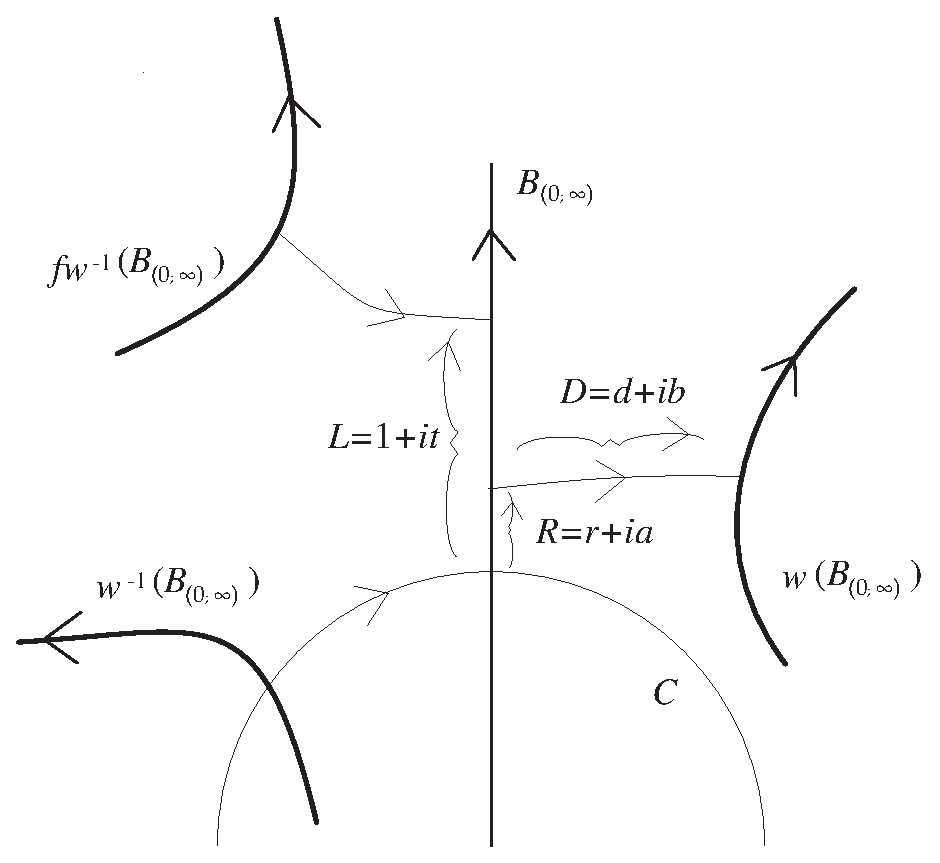
\includegraphics[scale=0.500]{fig1.1}
\end{figure}

\begin{definition}\label{GMT 1.12}
\hglue-8pt Let ${\mathcal P}\subset{\mathcal P}^{\prime}$ be the set of those parameters $\alpha
= (l+it$, $d+ib, r+ia)$ such
that
 \vglue3pt
 a)       $0.0978\le l \le 1.289785$,
\vglue2pt b)\enspace      $l/2 \le d\le \ln(3)$,
\vglue2pt c) \enspace   $0\le r \le l/2$,
\vglue2pt d) \enspace      $-\pi \le t \le 0$,
\vglue2pt e) \enspace	$-\pi \le b \le \pi$,
\vglue2pt f) \enspace	$-\pi \le a \le \pi$.
\vglue2pt\noindent 
Define ${\mathcal T}={\mathcal T}^{\prime}\cap {\mathcal P}.$
\end{definition}

The point of the definition of ${\mathcal P}$ and ${\mathcal T}$ is as follows.  We want to analyze by computer the relationship between lengths of shortest geodesics  and their tuberadii in hyperbolic $3$-manifolds.  We were naturally led to the parameter space 
${\mathcal P}^{\prime}$ and its subset ${\mathcal T}^{\prime}.$  But 
${\mathcal P}^{\prime}$ is problematic from the computational viewpoint because it is noncompact.  We wish to replace 
${\mathcal P}^{\prime}$ by ${\mathcal P}$ which is compact, and 
${\mathcal T}^{\prime}$ by ${\mathcal T}$ in our computer analysis.  This is carried out in Lemma \ref{GMT 1.13}.  Note that we worked to make ${\mathcal P}$ as small as reasonable to save computation time;  for example, the $t$ and $r$ restrictions above cut down the parameter space by a factor of 4 over the obvious $t$ and $r$ restrictions. 

\begin{lemma}\label{GMT 1.13}
If $\alpha=(l+it, d+ib, r+ia)\in {\mathcal T}^{\prime}$ has $d\le \ln(3)$ and
corresponds to a $2$\/{\textrm -}\/generator group
$\{G_\alpha,f_\alpha,w_\alpha\},$ then there exists a parameter $\beta=(l^{\prime}+it^{\prime}, d^{\prime}+ib^{\prime}, r^{\prime}+ia^{\prime})\in {\mathcal T}$ 
with associated group $\{G_\beta,f_\beta, w_\beta\}$ such that $G_\beta$ is conjugate (in ${\textrm Isom}({\mathbf H}^3$)) to $G_\alpha.$ 
\end{lemma}

\begin{proof} We note that $d < l/2$ is eliminated from consideration by Proposition 1.11 i), and the definition of ${\mathcal T}^\prime.$ If $d\le \ln(3),$
then
$0.0978\le l\le 1.289785$ by Propositions 1.10 and 1.11 ii).  If for the marked group $\{G, f, w\}$ we have 
$-l/2<r<0,$ then the marked group
$\{G,f,w^{-1}\}$ is conjugate to an element of ${\mathcal T}$ whose new
$r$-parameter is $-r.$  Thus we can assume that
conditions a, b, c from Definition 1.12 hold for the relevant $\{G,f,w\}.$  Further,    conditions e and f hold.

This leaves condition 1.12d.  Conjugating $G$ by a
reflection in the geodesic plane spanned
by $B_{(0;\infty)}$ and $B_{(-1;1)}$ changes the $t$-parameter to 
$-t \ ({\textrm mod}\ 2\pi)$
but leaves the $r$ and $d$ parameters unchanged.
The effect on $b$ and $a$ is irrelevant.  \end{proof}

By [G; Lemma 5.9] (or see Example A.3 in the appendix) a closed orientable hyperbolic $3$-manifold $N$
satisfies the insulator condition provided that
tuberadius$(\delta) > \ln(3)/2$ for some closed geodesic $\delta\subset N.$  Thus we
are led to consider:

\begin{definition}  A word $h$ in $w,f,w^{-1},f^{-1}$ for which statement a) (resp.\ b)) in Remark \ref{GMT 1.17} holds for each $\beta\in {\mathcal P}_i$
and for which $h_\beta$ is not a power of $f_\beta$ for each $\beta\in {\mathcal P}_i$ is
called a {\textit killerword} for ${\mathcal P}_i$ with respect to contradiction a) (resp.\ b)).
\end{definition}

\begin{summary}  With seven exceptions,  to each of the approximately one
billion regions partitioning ${\mathcal P},$ we will
associate a killerword and a contradiction.  \end{summary} 

\begin{remark}  Computers are well suited for partitioning a set such as ${\mathcal P}$
into many regions $\{{\mathcal P}_i \},$ and finding a
killerword $h_i$ which eliminates all $\alpha_i \in {\mathcal P}_i $ due to contradiction $C_i.$
Depending on the contradiction, we find
computable expressions  for approximations of the values of
$\Relength(h_\beta)$ or Redistance$(h_\beta(B_{(0;\infty)}), B_{(0;\infty)})$ and
thus use the computer to eliminate all of~${\mathcal P}_i .$ 
\end{remark}

\vglue8pt 
{\textit Definition} \ref{GMT 1.22}. Let 
\vglue4pt
\centerline{$ {\mathcal W} = \{ (x_0,x_1,x_2,x_3,x_4,x_5) : |x_i| \le 4 \times 2^{(5 - i) /6} {\mathrm \ for\ } i = 0,1,2,3,4,5 \}$}
\begin{eqnarray*}
\noalign{\vskip-12pt}
 \supset \exp({\mathcal P}) = 
\{(x_0,x_1,x_2,x_3,x_4,x_5)\mid \hskip-16pt&\hskip-16pt & 
x_0 + i x_3=\exp(e),  \enspace x_1 + i x_4
  = \exp(f),  \\
\hskip-16pt&\hskip-16pt& x_2 + i x_5 = \exp(g) \
{\textrm where} (e,f,g)\in {\mathcal P}\}\\
\noalign{\vskip-28pt}
\end{eqnarray*}
 and let
$${\mathcal S}=\exp({\mathcal T}).$$
As we are taking $\exp$ of the various complex co-ordinates, it is notationally convenient to replace our complex parameters 
$L = l+it,\ D = d+ib,\ R = r+ia$ by exponentiated versions.  That is, let 
\begin{eqnarray*}
L^\prime &\hskip-8pt=\hskip-8pt& \exp(L) = \exp(l+it),\enspace D^\prime = \exp(D) = \exp(d + ib), 
\\ R^\prime &\hskip-8pt=\hskip-8pt& \exp(R) = \exp(r+ia).
\end{eqnarray*}
 

{\textit Remarks} \ref{GMT 1.23}.
i) We work with ${\mathcal W}$ instead of $\exp({\mathcal P})$ because we want our initial parameter space to be a (6-dimensional) box that is easily
subdivided.  This has the side effect that certain regions (sub-boxes)
 ${\mathcal W}_i$ of ${\mathcal W}$ will be eliminated because they are outside of $\exp({\mathcal P})$ not because of the analogues of conditions a) and b) in
Remark \ref{GMT 1.17}.
The entire collection of conditions is given in Chapter FIXME(5).
 
ii)  The presence of the factor $2^{(5-i)/6}$ in the definition of ${\mathcal W}$ is explained in Construction \ref{GMT 5.3}.
Briefly, the main reason for including it
is to make the shape of regions stay as uniform and ``round" as possible under subdivision.
This makes the Taylor approximations efficient, hence fast.
\vglue4pt
iii)  We chose the co-ordinates of ${\mathcal W}$  so that $L^\prime = x_0 + i x_3,\ D^\prime = x_1 + i x_4,\ R^\prime = x_2 + i x_5\ $ to gain a mild
computer advantage.  

\begin{lemma}{}  If $(L^\prime, D^\prime, R^\prime)\in {\mathcal W}$ and  $\{G,f,w\}$ is the associated normalized 
marked group{\textrm ,} then $f$ and $w$ have matrix representatives
 $$ f = \left(
	\begin{matrix}
		\sqrt{L^\prime}&0\cr
		0 & 1/\sqrt{L^\prime}\cr
	\end{matrix}
	\right), \leqno{{\mathrm a)}}$$

	$$ w = \left(\begin{matrix}
		\sqrt{R^\prime} * ch & \sqrt{R^\prime} * sh \cr
		sh / \sqrt{R^\prime} & ch/\sqrt{R^\prime}\cr
	\end{matrix}
	\right) \leqno{\mathrm b)}$$ 
where 
$ch = (\sqrt{D^\prime} + 1/\sqrt{D^\prime})/2\ \ {\textrm and}\ \ 
sh = (\sqrt{D^\prime} - 1/\sqrt{D^\prime})/2.$
\end{lemma}
 
\begin{proof}{}  a)  In our set-up  the (oriented) axis of $f$ is $B_{(0;\infty)}$.  
As such, $f$ corresponds to a diagonal matrix, with diagonal entries $p$ and $p^{-1},$  with $|p| >1.$ 
The action of $f$ on the bounding complex plane is simply multiplication by $p^2.$  Extending this action to upper-half-space in the natural way rotates the $z$-axis by angle $\arg(p^2)$ and sends $(0,0,1)$ to $(0,0,|p|^2).$ 
 Thus, $${\mathrm Im}(\length(f)) = \arg(p^2) = {\mathrm Im}(\ln(p^2))$$ and,
using the hyperbolic metric, 
$${\mathrm Re}(\length(f)) = \ln(|p|^2) = {\mathrm Re}(\ln(p^2)).$$
That is, $\length(f) = \ln(p^2)$ and 
$$p = \pm \exp(\length(f)/2) = \pm \sqrt{\exp(\length(f))} = \pm \sqrt{\exp(L)} = \pm \sqrt{L^\prime}.$$ Now, we take the positive square
root (taking the negative square root produces the other lift from 
${\textrm PSL(2,}{\mathbf C})$ to ${\mathrm SL(2,}{\mathbf C})$).

b)  $w = \beta \circ \alpha$ where $\beta$ is translation of distance $R$ along $ B_{(0;\infty)}$ and $\alpha$ is translation of distance $D$ along $ B_{(-1;1)}$.  Thus,
	a matrix representative of $\beta$ is $$ \left(\begin{matrix}\sqrt{R^\prime} & 0 \cr 0 & 1/\sqrt{R^\prime}\cr\end{matrix}\right)$$ and a matrix representative of $\alpha$ can be computed to be $$\left(\begin{matrix}\cosh(D/2) & \sinh(D/2) \cr \sinh(D/2) & \cosh(D/2)\cr\end{matrix}\right).$$ But
$\cosh(D/2) = (\exp(D/2) + \exp(-D/2))/2 = 
(\sqrt{D^\prime} + 1/\sqrt{D^\prime})/2 = ch$ and similarly for $sh.$
Thus, $$\alpha = \left(\begin{matrix}ch & sh \cr sh & ch\cr\end{matrix}\right)$$ and b) follows by matrix multiplication.
\end{proof}

\begin{lemma}{} If $h \in {\textrm Isom}_+({\mathbf H}^3)$ is represented by the matrix $$A = \left(\begin{matrix}a &  b \cr c & d\cr\end{matrix}\right)\in {\mathrm SL}(2,{\mathbf
C}),$$ then 
\begin{itemize}
\item{a)} $\exp(\Relength (h))= |\trace(A)/2 \pm \sqrt{(\trace(A)/2)^2 - 1}|^2,$

\item{b)} $\exp({\textrm Redistance} (h(B_{(0;\infty)}), B_{(0;\infty)}))=|{\textrm orthotrace}(A) \pm$\hfill \noindent $\sqrt{({\mathrm
orthotrace}(A))^2 - 1}|$  where 
{\textrm orthotrace(}$A) = ad + bc.$ $\phantom{\sum^\int}$
\end{itemize}
In both cases{\textrm ,} the $+, -$ produce reciprocal values for the right\/{\textrm -}\/hand side{\textrm ,}
  and we take the one producing the larger value{\textrm ,} unless the value is $1${\textrm ,} in
which case there is no need to choose.
\end{lemma}

\begin{proof}{}  a)  If $A$ is elliptic or parabolic, the proof is straightforward (the trace of a parabolic is $\pm 2$ while the trace of an elliptic
is a real number between 2 and -2).  

We assume $A$ is hyperbolic.  Because trace is a conjugacy invariant, we can assume the oriented axis of $A$ is $ B_{(0;\infty)}.$  Thus $A$ is a diagonal matrix with $p$ and $p^{-1}$ along the diagonal with 
$|p| > 1,$ and, as in the proof of Lemma \ref{GMT 1.24}, we see that 
$\exp({\textrm length}(h)) = p^2.$  Of course,  $\trace(A)= p + p^{-1}$, and it is easy enough to solve for $p.$   Specifically, 
$p = \trace(A)/2 \pm \sqrt{(\trace(A)/2)^2 - 1}.$
Thus, 
\begin{eqnarray*}
\exp(\Relength (h))& =& |\exp(\length(h))|  = 
|p|^2\\[5pt]
&=& |(\trace(A)/2) \pm \sqrt{(\trace(A)/2)^2 - 1}|^2.
\end{eqnarray*}
\vglue4pt
b)  If $ B_{(0;\infty)}$ and $h(B_{(0;\infty)})$ intersect at infinity, then the proof is straightforward.  For example, 
if $h$ fixes the point $(0,0,0)$ at infinity, then $c = 0,\ ad = 1$ and the formula holds.  Similarly for the other cases in which $ B_{(0;\infty)}$ and $h(B_{(0;\infty)})$ intersect at infinity.

We assume $ B_{(0;\infty)}$ and $h(B_{(0;\infty)})$ do not intersect at infinity. We will compute the length of $k$, the square of the transformation taking $ B_{(0;\infty)}$ to $h(B_{(0;\infty)})$ along their ortholine. 
Let $\tau$ be 180-degree rotation about $ B_{(0;\infty)},$ then $(h \circ \tau \circ h^{-1})$ is 180-degree rotation about $h(B_{(0;\infty)}),$ and
we have that  $k = (h \circ \tau \circ h^{-1}) \circ \tau.$   
Now, $\tau$ and $h$ are represented by the matrices 
$$ \left(\begin{matrix} i & 0 \cr 
0  & -i \cr\end{matrix} \right) {\mathrm \ \ and\ \ } 
                         \left(\begin{matrix} a & b \cr 
			 c  & d \cr\end{matrix} \right)  \in {\mathrm SL}(2,{\mathbf C}).$$ 
Hence,   $k = (h \circ \tau \circ h^{-1}) \circ \tau$ can be computed to have matrix
representation $$\left(\begin{matrix} ad + bc & 2ab \cr 
2cd & ad + bc \cr\end{matrix} \right).$$ 
Thus,
\begin{eqnarray*}
&&\hskip-66pt\exp({\textrm Redistance} (h(B_{(0;\infty)}), B_{(0;\infty)}))\\
& = &
\exp(\Relength(k)/2)= \sqrt{|\exp(\length(k)|}\\
& =&
|(\trace(k)/2) \pm \sqrt{(\trace(k)/2)^2 - 1}|\\
& =&
|(ad + bc) \pm \sqrt{(ad + bc)^2 - 1}|. \\
\noalign{\vskip-36pt}
\end{eqnarray*}
\end{proof}

\begin{remark} i)  It follows from Lemma \ref{GMT 1.25} that if $h$ is a word in $f,w,f^{-1},w^{-1},$ then for any
parameter value $\alpha\in {\mathcal W},$
$$\exp(\Relength(h_\alpha)), \hbox{ and }
  \exp({\textrm Redistance}(h_\alpha(B_{(0;\infty)}), B_{(0;\infty)}))$$ can be computed using only the
operations $+, -, \times, /, \sqrt{}.$
\vglue4pt
\end{remark} %FIXME
 ii) During the course of the computer work needed to prove the main theorems, the parameter space
${\mathcal W}$ was decomposed into sub-boxes by computer via a recursive subdivision process:
Given a sub-box  being analyzed, either it can be {\textit killed directly} (that is, eliminated by a killerword and associated condition as described in
Remark \ref{GMT 1.17},
or for the trivial reason described in Remark FIXME(1.23i)), or it cannot.  
If it cannot be killed directly, it is subdivided in half by a hyperplane
$\{x_i = c \}$ (where $i$ runs through the various co-ordinate dimensions
cyclically) and the two pieces are analyzed separately, and so on. 

As such, a sub-box of ${\mathcal W}$ can be described by a sequence of 0's and 1's where 0 means ``take the lesser $x_i$ values" and 1 means ``take the greater $x_i$ values."  
For the decomposition of ${\mathcal W}$ into sub-boxes, all the 
sub-box descriptions could be neatly encoded into one tree (although in practice we found it preferable to use several trees to describe the entire
decomposition.  See \S 5).
\vglue4pt
iii) In the following proposition, seven {\textit exceptional boxes} are described as sequences of 0's and 1's.  
Four of the exceptional boxes---$X_0, X_4, X_5, X_6$---are each the union of two abutting sub-boxes, $X_0 = X_{0a} \cup X_{0b}$ and so on.  It is a pleasant exercise to work through the fact that they abut.  
It should be noted that had the set-up for ${\mathcal W}$ been different, more sub-boxes (or perhaps fewer) might have been needed to construct the seven
exceptional regions. 

It is also a pleasant exercise to calculate by hand the co-ordinate ranges of the various sub-boxes.  For example, the range of the last co-ordinate (i.e., $x_5$) of the sub-box 
\eject

\noindent 
$X_{6a} = 
111000000001000111\ 
111111110101001111\ 
011111010111111111$\hfill
\vglue4pt
  \hfill $  
110001001011000111\ 0$
\vglue4pt\noindent 
is found by taking the 6th entry, the 12th entry, the 18th entry, and so on.  These entries are 011111111111.  The first entry (0) means take the
lesser $x_5$ values, and produces the interval $[-4,0].$  The second entry (1) means take the greater $x_5$ values, and produces the interval
$[-2,0].$  The third entry (1) produces $[-1,0].$  Continuing, we see that $X_{6a}^{\phantom{|}}$ has $-2^{-9} \le x_5 = {\mathrm Im}(R') \le 0.$  The other
co-ordinates can be computed in the same fashion, although they must at the end be multiplied by the factor $2^{(5 - i)/6}$ (see the definition of the
initial box
${\mathcal W}$).  The range of co-ordinate values for each  exceptional  box $X_0, X_1, \ldots, X_6$ is given in Table \ref{GMT tab 1.1} (a limited number of significant
digits is given), and  then a range of co-ordinates for exceptional regions (in ${\mathcal P}$) 
${\mathcal R}_i \supset \exp^{-1}(X_i)$ is given (see Remarks FIXME:1.30i) and 1.30ii)) in Table \ref{GMT tab 1.2}. (Note that this use of the symbol ${\mathcal R}_i$ differs
slightly from the use in \S 0.)
Finally, two {\textit quasi-relators} are given in Proposition \ref{GMT 1.28} for each exceptional box $X_0, X_1, \ldots, X_6$ (see the next definition).
 
\begin{table}\label{GMT tab 1.1}
\caption{Exceptional boxes in $(L',D',R')$ co-ordinates in ${\mathcal W}$; truncated values}
 
\begin{small}
$$
\begin{array}{rlrlrlrl}
\noalign{\noindent $X_0$}
\noalign{\vskip2pt}
l'_{\textrm min} &\hskip-6pt = -0.84065&\enspace l'_{\textrm max} &\hskip-6pt = -0.84060&\enspace
t'_{\textrm min}&\hskip-6pt = -2.13726&\enspace t'_{\textrm max}&\hskip-6pt = -2.13722\\
 d'_{\textrm min}&\hskip-6pt = -0.84064& d'_{\textrm max} &\hskip-6pt = -0.84059&
b'_{\textrm min}&\hskip-6pt = -2.13729& b'_{\textrm max} &\hskip-6pt = -2.13722\\
r'_{\textrm min} &\hskip-6pt = 0.999979& r'_{\textrm max} &\hskip-6pt = 1.000022&
a'_{\textrm min}&\hskip-6pt = -0.00006103& a'_{\textrm max}&\hskip-6pt = 0.00006103\end{array}
$$
$$
\begin{array}{rlrlrlrl}
\noalign{\vskip2pt}
\noalign{ \noindent $X_1$}
\noalign{\vskip2pt}
l'_{\textrm min} &\hskip-6pt = -1.34852&\enspace  l'_{\textrm max} &\hskip-6pt = -1.34831&\enspace 
t'_{\textrm min} &\hskip-6pt = -2.66102&\enspace  t'_{\textrm max} &\hskip-6pt = -2.66072\\
d'_{\textrm min} &\hskip-6pt = -0.54334& d'_{\textrm max}
&\hskip-6pt = -0.54315&   b'_{\textrm min} &\hskip-6pt = -2.85877&  b'_{\textrm max} &\hskip-6pt = -2.85849\\
r'_{\textrm min} &\hskip-6pt = 0.90390& 
r'_{\textrm max} &\hskip-6pt = 0.90408&   a'_{\textrm min} &\hskip-6pt = -1.47167&  a'_{\textrm max} &\hskip-6pt = -1.47143
\end{array}
$$
$$
\begin{array}{rlrlrlrl}
\noalign{\vskip2pt}
\noalign{\noindent $X_2$}
\noalign{\vskip2pt}
l'_{\textrm min} &\hskip-6pt =  -1.78701&\enspace   l'_{\textrm max} &\hskip-6pt =  -1.78527&\enspace  
t'_{\textrm min} &\hskip-6pt =  -2.27253&\enspace   t'_{\textrm max} &\hskip-6pt =  -2.27130\\
d'_{\textrm min} &\hskip-6pt =  -1.07428& d'_{\textrm max}
&\hskip-6pt =  -1.07273&   b'_{\textrm min} &\hskip-6pt =  -2.71846&  b'_{\textrm max} &\hskip-6pt =  -2.71736\\
r'_{\textrm min} &\hskip-6pt =  0.74163& 
r'_{\textrm max} &\hskip-6pt =  0.74301&   a'_{\textrm min} &\hskip-6pt =  -1.52929&  a'_{\textrm max} &\hskip-6pt =  -1.52832
\end{array}
$$

$$
\begin{array}{rlrlrlrl}
\noalign{\noindent 
$X_3$}
\noalign{\vskip2pt} l'_{\textrm min} &\hskip-6pt =   0.58117&\enspace   l'_{\textrm max} &\hskip-6pt =   0.58160&\enspace  
t'_{\textrm min} &\hskip-6pt =   -3.31221&\enspace   t'_{\textrm max} &\hskip-6pt =   -3.31190\\
d'_{\textrm min} &\hskip-6pt =   1.15644& d'_{\textrm max}
&\hskip-6pt =   1.15683&  b'_{\textrm min} &\hskip-6pt =   -2.75628& b'_{\textrm max} &\hskip-6pt =   -2.75573\\
r'_{\textrm min} &\hskip-6pt =   1.40420&
r'_{\textrm max} &\hskip-6pt =   1.40454&  a'_{\textrm min} &\hskip-6pt =   -1.17968& a'_{\textrm max} &\hskip-6pt =   -1.17919
\end{array}
$$
$$
\begin{array}{rlrlrlrl}
\noalign{\noindent 
$X_4$}
\noalign{\vskip2pt}
l'_{\textrm min} &\hskip-6pt = 0.33321&\enspace   l'_{\textrm max} &\hskip-6pt = 0.33495&\enspace  
t'_{\textrm min} &\hskip-6pt = -3.31959&\enspace   t'_{\textrm max}&\hskip-6pt = -3.31898\\
d'_{\textrm min} &\hskip-6pt = 0.97739& d'_{\textrm max}
&\hskip-6pt = 0.97817&  b'_{\textrm min} &\hskip-6pt = -2.82533& b'_{\textrm max} &\hskip-6pt = -2.82478\\
r'_{\textrm min} &\hskip-6pt = 1.35413&
r'_{\textrm max} &\hskip-6pt = 1.35482&  a'_{\textrm min} &\hskip-6pt = -1.22558& a'_{\textrm max} &\hskip-6pt = -1.22460\end{array}$$
$$\begin{array}{rlrlrlrl}
\noalign{\noindent 
$X_5$}
\noalign{\vskip2pt}
l'_{\textrm min} &\hskip-6pt = -1.37984&\enspace   l'_{\textrm max}&\hskip-6pt = -1.37810&\enspace  
t'_{\textrm min} &\hskip-6pt = -2.53706&\enspace   t'_{\textrm max} &\hskip-6pt = -2.53460\\
d'_{\textrm min} &\hskip-6pt = -1.37967& d'_{\textrm max}
&\hskip-6pt = -1.37657&  b'_{\textrm min}&\hskip-6pt = -2.53650& b'_{\textrm max} &\hskip-6pt = -2.53430\\
r'_{\textrm min} &\hskip-6pt = 0.99989&
r'_{\textrm max} &\hskip-6pt = 1.00265&  a'_{\textrm min} &\hskip-6pt = -0.001953& a'_{\textrm max} &\hskip-6pt = 0.001953\end{array}$$

$$\begin{array}{rlrlrlrl}
\noalign{\noindent 
$X_6$}
\noalign{\vskip2pt}
l'_{\textrm min} &\hskip-6pt = 1.37810&\enspace   l'_{\textrm max}&\hskip-6pt = 1.37984&\enspace  
t'_{\textrm min} &\hskip-6pt = -2.53706&\enspace   t'_{\textrm max} &\hskip-6pt = -2.53460\\
d'_{\textrm min} &\hskip-6pt = 1.37657& d'_{\textrm max}
&\hskip-6pt = 1.37967& b'_{\textrm min} &\hskip-6pt = -2.53650& b'_{\textrm max}&\hskip-6pt = -2.53430\\
r'_{\textrm min} &\hskip-6pt = 0.99989&
r'_{\textrm max} &\hskip-6pt = 1.00265&  a'_{\textrm min} &\hskip-6pt = -0.001953& a'_{\textrm max} &\hskip-6pt = 0.001953
\end{array}$$
\end{small}
 \vglue12pt
 \end{table}

\begin{table}\label{GMT tab 1.2}
\caption{Exceptional regions (boxes) in $(L,D,R)$ co-ordinates in ${\mathcal P}$}
\begin{small}
$$
\begin{array}{rlrl}
\noalign{\noindent  ${\mathcal R}_0$}
\noalign{\vskip2pt}
l_{\textrm min} &\hskip-6pt =  0.8314&\enspace    l_{\textrm max}&\hskip-6pt  = 0.8315\\
t_{\textrm min} &\hskip-6pt =  -1.9456&\enspace    t_{\textrm max}&\hskip-6pt  = -1.9455\\
d_{\textrm min} &\hskip-6pt =  0.8314&  d_{\mathrm
max}&\hskip-6pt  = 0.8315\\   b_{\textrm min} &\hskip-6pt =  -1.9456&  b_{\textrm max} &\hskip-6pt = -1.9455\\
r_{\textrm min} &\hskip-6pt =  -0.00002051&  r_{\textrm max} &\hskip-6pt = 0.00002267\\  a_{\textrm min} &\hskip-6pt =  -0.00006105&  a_{\mathrm
max}&\hskip-6pt  = 0.00006105\end{array}
$$

%$$
%\begin{array}{rlrlrlrl}
%\noalign{\noindent  ${\mathcal R}_0$}
%\noalign{\vskip2pt}
%l_{\textrm min} &\hskip-6pt =  0.8314&\enspace    l_{\textrm max}&\hskip-6pt  = 0.8315&\enspace   
%t_{\textrm min} &\hskip-6pt =  -1.9456&\enspace    t_{\textrm max}&\hskip-6pt  = -1.9455\\
%d_{\textrm min} &\hskip-6pt =  0.8314&  d_{\mathrm
%max}&\hskip-6pt  = 0.8315&   b_{\textrm min} &\hskip-6pt =  -1.9456&  b_{\textrm max} &\hskip-6pt = -1.9455\\
%r_{\textrm min} &\hskip-6pt =  -0.00002051&  r_{\textrm max} &\hskip-6pt = 0.00002267&   a_{\textrm min} &\hskip-6pt =  -0.00006105&  a_{\mathrm
%max}&\hskip-6pt  = 0.00006105\end{array}
%$$


$$\begin{array}{rlrlrlrl}
\noalign{\noindent  ${\mathcal R}_1$}
\noalign{\vskip2pt}
l_{\textrm min} &\hskip-6pt =  1.0928&\enspace    l_{\textrm max} &\hskip-6pt = 1.0931&\enspace   
t_{\textrm min} &\hskip-6pt =  -2.0399&\enspace   t_{\textrm max}&\hskip-6pt  = -2.0397\\
d_{\textrm min} &\hskip-6pt =  1.0680&  d_{\mathrm
max}&\hskip-6pt  = 1.0682&   b_{\textrm min} &\hskip-6pt =  -1.7587&  b_{\textrm max} &\hskip-6pt = -1.7585\\
r_{\textrm min} &\hskip-6pt =  0.5463& 
r_{\textrm max}&\hskip-6pt  = 0.5465&   a_{\textrm min} &\hskip-6pt =  -1.0201&  a_{\textrm max}&\hskip-6pt  = -1.0198\end{array}$$

$$\begin{array}{rlrlrlrl}\noalign{\noindent  ${\mathcal R}_2$}
\noalign{\vskip2pt}
l_{\textrm min} &\hskip-6pt =  1.0608&\enspace    l_{\textrm max} &\hskip-6pt = 1.0617&\enspace   
t_{\textrm min} &\hskip-6pt =  -2.2375&\enspace    t_{\textrm max} &\hskip-6pt = -2.2366\\
d_{\textrm min} &\hskip-6pt =  1.0720&  d_{\mathrm
max}&\hskip-6pt  = 1.0727&   b_{\textrm min} &\hskip-6pt =  -1.9473&  b_{\textrm max} &\hskip-6pt = -1.9466\\
r_{\textrm min} &\hskip-6pt =  0.5298& 
r_{\textrm max} &\hskip-6pt = 0.5308&   a_{\textrm min} &\hskip-6pt =  -1.1193&  a_{\textrm max} &\hskip-6pt = -1.1182\end{array}$$

$$\begin{array}{rlrlrlrl}
\noalign{\noindent  ${\mathcal R}_3$}
\noalign{\vskip2pt}
l_{\textrm min} &\hskip-6pt =  1.2126&\enspace    l_{\textrm max} &\hskip-6pt = 1.2129&\enspace   
t_{\textrm min} &\hskip-6pt =  -1.3972&\enspace    t_{\textrm max}&\hskip-6pt  = -1.3969\\
d_{\textrm min} &\hskip-6pt =  1.0947&  d_{\mathrm
max}&\hskip-6pt  = 1.0951&   b_{\textrm min} &\hskip-6pt =  -1.1736&  b_{\textrm max}&\hskip-6pt  = -1.1733\\
r_{\textrm min} &\hskip-6pt =  0.6063& 
r_{\textrm max}&\hskip-6pt  = 0.6067&   a_{\textrm min} &\hskip-6pt =  -0.6988&  a_{\textrm max}&\hskip-6pt  = -0.6984\end{array}
$$

$$\begin{array}{rlrlrlrl}
\noalign{\noindent  ${\mathcal R}_4$}
\noalign{\vskip2pt}
l_{\textrm min} &\hskip-6pt =  1.2046&\enspace    l_{\textrm max}&\hskip-6pt  = 1.2050&\enspace   
t_{\textrm min} &\hskip-6pt =  -1.4708&\enspace    t_{\textrm max}&\hskip-6pt = -1.4702\\
d_{\textrm min} &\hskip-6pt =  1.0949&  d_{\mathrm
max}&\hskip-6pt  = 1.0953&   b_{\textrm min} &\hskip-6pt =  -1.2378&  b_{\textrm max} &\hskip-6pt = -1.2374\\
r_{\textrm min} &\hskip-6pt =  0.6019& 
r_{\textrm max} &\hskip-6pt = 0.6027&   a_{\textrm min} &\hskip-6pt =  -0.7357&  a_{\textrm max} &\hskip-6pt = -0.7349\end{array}$$

$$\begin{array}{rlrlrlrl}
\noalign{\vskip-10pt}
\noalign{\noindent  ${\mathcal R}_5$}
\noalign{\vskip2pt}
l_{\textrm min} &\hskip-6pt =  1.0595&\enspace    l_{\textrm max}&\hskip-6pt = 1.0606&\enspace   
t_{\textrm min}&\hskip-6pt =  -2.0694&\enspace   t_{\textrm max} &\hskip-6pt = -2.0683\\
d_{\textrm min} &\hskip-6pt =  1.0591&  d_{\mathrm
max}&\hskip-6pt  = 1.0604&   b_{\textrm min} &\hskip-6pt =  -2.0694&  b_{\textrm max}&\hskip-6pt  = -2.0680\\
r_{\textrm min} &\hskip-6pt =  -0.0001069&  r_{\textrm max} &\hskip-6pt =  0.002654&  a_{\textrm min} &\hskip-6pt =  -0.001954&  a_{\textrm max}
&\hskip-6pt =  0.001954\end{array}$$

$$\begin{array}{rlrlrlrl}
\noalign{\noindent  ${\mathcal R}_6$}
\noalign{\vskip2pt}
l_{\textrm min} &\hskip-6pt =  1.0595&\enspace    l_{\textrm max} &\hskip-6pt =  1.0606&\enspace   
t_{\textrm min} &\hskip-6pt =  -1.0733&\enspace    t_{\textrm max} &\hskip-6pt =  -1.0722\\
d_{\textrm min} &\hskip-6pt =  1.0591&  d_{\textrm max}
&\hskip-6pt =  1.0604&   b_{\textrm min} &\hskip-6pt =  -1.0736&  b_{\textrm max} &\hskip-6pt =  -1.0722\\
r_{\textrm min} &\hskip-6pt =  -0.0001069& 
r_{\textrm max} &\hskip-6pt =  0.002654&   a_{\textrm min} &\hskip-6pt =  -0.001954&  a_{\textrm max} &\hskip-6pt =  0.001954\end{array}$$
\end{small}
\end{table}

\begin{definition} A {\textit quasi-relator} in a sub-box $X$ of ${\mathcal W}$ is a word in $f,w,F=f^{-1},W=w^{-1}$ that is close to the identity
throughout
$X$ and experimentally appears to be converging to the identity at some point in $X.$  In particular, a quasi-relator rigorously has Relength less than
that of $f$ at all points in $X.$
\end{definition}

\begin{proposition}\label{GMT 1.28}  
Within the parameter space ${\mathcal W}$ but outside the seven exceptional boxes there are no parameter points corresponding to 
marked groups $\{G,f,w\}$ where $G$ is 
discrete{\textrm ,} torsion\/{\textrm -}\/free and  parabolic\/{\textrm -}\/free\/{\textrm ;}
$f$ corresponds to a shortest geodesic $\delta$ of tuberadius $\le
\ln(3)/2${\textrm ;} and $w$ takes a particular lift of $\delta$ to 
a nearest translate.
 Specifically{\textrm ,} 
${\mathcal S} \cap ({\mathcal W} - \bigcup_{n = 0,\dots, 6} X_n)=\emptyset$ where the $X_n$ are the exceptional boxes

\vglue4pt

 \noindent $X_0 = X_{0a} \cup X_{0b},$
\vglue8pt
\noindent $X_{0a} = 
001000110111110001\ 
101001010101011001\ 
011011010111101101$\hfill 

 
 \hfill
$100001101101000111\ 
010001110101100101\ 
1101110111110100,$  
\vglue8pt
 \noindent $X_{0b} = 
001001110110110000\ 
101000010100011000\ 
011010010110101100$

\hfill
$100000101100000110\ 
010000110100100100\ 
1101100111100100,$ 
 \vglue4pt
\noindent  $X_0\ \ $ quasi\/{\textrm -}\/relators\/{\textrm :}

$r_1 = fwFwwFwfww,$
 
$r_2 = FwfwfWfwfw,$

\vglue8pt
\noindent $X_1 = 
001000110001110110\ 
011101000110111110\ 
100010110000100011$\hfill 

\hfill $
101101001101001000\ 
110101011000000100\ 
000.$ 

\noindent $X_1\ \ 
$ quasi\/{\textrm -}\/relators\/{\textrm :}

$r_1 = FFwFWFWfWFWFwFFww,$
 
$r_2 = FFwwFwfwfWfwfwFww,$
\vglue4pt
\noindent $X_2 = 
001000110101010010\ 
101010110001100101\ 
110111100001101010$\hfill

\hfill $111100100000010001\ 
111100,$
\vglue4pt
\noindent $X_2\ \ $ quasi\/{\textrm -}\/relators\/{\textrm :}

$r_1 = FwfwfWffWfwfwFww,$

$r_2 = FFwFFwwFwfwfwFww,$
\vglue4pt
\noindent 
$X_3 = 
111000000001000110\ 
011011101101011000\ 
111101011110001100$\hfill

\hfill  
$111111100110110000\ 
0000100010100010,$
\vglue4pt
\noindent $X_3\ \ $ quasi\/{\textrm -}\/relators\/{\textrm :}\/

$r_1 = FFwfwFFwwFWFwFWfWFWffWFWfWFwFWFww,$ 

$r_2 = FFwfwFwfWfwfWWfwfWfwFwfwFFwwFWFww,$
\vglue4pt 
\noindent $X_4 = X_{4a} \cup X_{4b},$
\vglue4pt
\noindent $X_{4a} = 
111000000001000110\ 
011001001111101010\ 
011110110110111101$\hfill

\hfill  
$100011111110110110\ 
10000111101,$
\vglue4pt
\noindent $X_{4b} = 
111000000001000110\ 
011001001111101010\ 
111110010110011101$\hfill

\hfill  
$000011011110010110\ 
00000101101,$
\vglue4pt
\noindent $X_4\ \ $ quasi\/{\textrm -}\/relators\/{\textrm :}

$r_1 = FFwfwFwfWfwfWfwFwfwFFwwFWFwFWFww,$

$r_2 = FFwfwFwfwFFwwFWFwFWfWFWfWFwFWFww,$
\vglue4pt
\noindent $X_5 = X_{5a} \cup X_{5b},$
\vglue4pt
\noindent $X_{5a} = 
001000110001110111\ 
001111000101111111\ 
101111100111001111$\hfill

\hfill 
$000001111011110111\ 1,$
\vglue4pt
\noindent  $X_{5b} = 
001001110000110110\ 
001110000100111110\ 
101110100110001110$\hfill

\hfill  
$000000111010110110\ 1,$
\vglue4pt
\noindent $X_5\ \ $ quasi\/{\textrm -}\/relators\/{\textrm :}

$r_1 = FwFWFwFwfwfWfwfw,$

$r_2 = FwfwfWfWFWfWfwfw,$
\vfil
\noindent $X_6 = X_{6a} \cup X_{6b},$
\vfil
\noindent $X_{6a} = 
111000000001000111\ 
111111110101001111\ 
011111010111111111$\hfill

\hfill  
$110001001011000111\ 0,$
\vglue4pt

\noindent $X_{6b} = 
111001000000000110\ 
111110110100001110\ 
011110010110111110$\hfill

\hfill  
$110000001010000110\ 0,$
\vglue4pt
\noindent $X_6\ \ $ quasi\/{\textrm -}\/relators\/{\textrm :}\/

$r_1 = FWFwFWfWFwFWFwfw,$

$r_2 = FWFwfwFwfWfwFwfw.$
\end{proposition}

 
\begin{proof}{}  
The proof follows along the lines presented in Remark \ref{GMT 1.17}.  
Two computer files contain the data needed for the proof.   
The first computer file describes the partition of ${\mathcal W}$ into
sub-boxes and attaches an integer to each such sub-box, 
and the second file, called ``conditionlist" is an ordered list of conditions and killerwords.
The integer associated to a sub-box in the first file describes the numbered condition/killerword from   conditionlist that will eliminate the sub-box
in question (other than those corresponding to the $X_i).$ A computer program named {\textit verify} shows
that the conditions and killerwords in question actually do kill off their associated sub-boxes (see Section 5 for more details).  This computer
program addresses the issues of Remark \ref{GMT 1.20}.  The code for {\textit
verify} is available at the {\textit Annals} web site. 

In addition, a mild modification of {\textit verify} showed that the listed words were quasi-relators for the given sub-boxes. 
\end{proof}


